\documentclass[border=1cm,10pt]{standalone}
\usepackage{tikz}
\usetikzlibrary{arrows}
\usetikzlibrary{decorations.pathmorphing}
\usetikzlibrary{decorations.markings}
\usetikzlibrary{patterns}

\definecolor{lyellow}{RGB}{244,244,150}


\tikzset{
      boson/.style={decorate, decoration={snake}, draw=black, line width=1.2},
      higgs/.style={dashed, draw=red, line width=1.2},
      lepton/.style={draw=blue, line width=1.2, postaction={decorate},
            decoration={markings,mark=at position .55 with {\arrow[draw=blue]{>}}}},
      alepton/.style={draw=blue, line width=1.2,  postaction={decorate},
            decoration={markings,mark=at position .55 with {\arrow[draw=blue]{<}}}},
      quark/.style={draw=blue, line width=1.2,  postaction={decorate},
            decoration={markings,mark=at position .55 with {\arrow[draw=blue]{>}}}},
      aquark/.style={draw=blue, line width=1.2,  postaction={decorate},
            decoration={markings,mark=at position .55 with {\arrow[draw=blue]{<}}}},
}


\begin{document}

    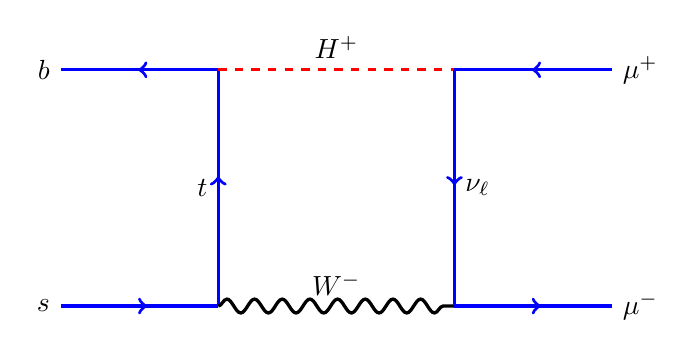
\begin{tikzpicture}
        % 

        % Draw the quarks
        \draw[quark] (0,0) node[left] {$s$} -- (2,0) ;
        \draw[aquark] (0,3) node[left] {$b$} -- (2,3) ;
        \draw[quark] (2,0) -- (2,3) node[midway,left] {$t$};

        \draw[boson] (2,0) -- (5,0) node[midway,above] {$W^{-}$} ;
        \draw[higgs] (2,3) -- (5,3) node[midway,above] {$H^{+}$} ;

        \draw[aquark] (5,0) -- (5,3) node[midway,right] {$\nu_{\ell}$};
        \draw[aquark] (5,3) -- (7,3) node[right] {$\mu^{+}$};
        \draw[quark] (5,0) -- (7,0) node[right] {$\mu^{-}$};

    \end{tikzpicture}

\end{document} 


